\begin{proposition}{5.2.2}
	Der er et unikt $p \in \so (A)$ som er tættest på $b$. Altså
	\[
		\norm{b-y} > \norm{b-p}
	\]
	hvor $y, p \in \so(A)$ og $y \not= p$.
\end{proposition}

\begin{bevis}
	Beviset for at $p$ er unik er som følger. Enhver vektor $b \in
	\mathbb{R}^m$ kan beskrives som
	\[
		b = p + z
	\]
	hvor $p \in \so(A)$ og $z \in (\so(A))^\bot$. Givet en vektor $y \in
	\so(A)$ forskellig fra $p$ gælder
	\[
		\norm{b-y}^2 = \norm{(b-p)+(p-y)}^2
	\]
	\begin{center}
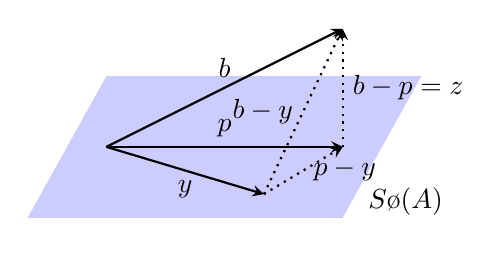
\begin{tikzpicture}
	\tikzset{>=stealth}
	\fill[blue!20] (0,0) -- (1,1.8) -- (5,1.8) -- (4,0) -- cycle;

	\node (sa) at (4.8,0.2) {$S\text{ø}(A)$};

	\coordinate (s) at (1,0.9);
	\coordinate (pE) at (4,0.9);
	\coordinate (bE) at (4,2.4);
	\coordinate (yE) at (3,0.3);
	
	\draw[thick,->] (s) to node[above]{$p$} (pE);
	\draw[thick,->] (s) to node[above]{$b$} (bE);
	\draw[thick,->,dotted] (pE) to node[right]{$b-p = z$} (bE);
	\draw[thick,->] (s) to node[below]{$y$} (yE);
	\draw[thick,->,dotted] (yE) to node[left]{$b-y$} (bE);
	\draw[thick,->,dotted] (yE) to node[right]{$p-y$} (pE);
\end{tikzpicture}
\end{center}

	da $p-y \in \so(A)$ og $b-p = z \in (\so(A))^\bot$ så får vi fra Pythagoras
	\[
		\norm{b-y}^2 = \norm{b-p}^2 + \norm{p-y}^2
	\]
	og vi kan derfor konkludere at
	\[
		\norm{b-y} > \norm{b-p}
	\]
\end{bevis}
